%%
%% Author: gdidot
%% 7/13/18
%%

% Preamble
\documentclass[11pt, a4paper, pdftex]{article}

% Packages
\usepackage[a4paper,top=3cm,bottom=2cm,left=3cm,right=3cm,marginparwidth=1.75cm,head=61pt]{geometry}
\usepackage{a4wide}
\usepackage[french]{babel}
\usepackage[utf8]{inputenc}
\usepackage{graphicx}
\usepackage{fancyhdr}
\usepackage{lastpage}
\usepackage[T1]{fontenc}
\usepackage[toc,page]{appendix}
\usepackage{caption}
\usepackage[hidelinks, colorlinks = true, urlcolor = blue, linkcolor = black]{hyperref}

\renewcommand{\appendixtocname}{Annexes}
\renewcommand{\appendixpagename}{Annexes}

\newcommand{\info}{\texttt}

% Document
\begin{document}

    %Info pour maketitle
    \title{Rapport de Stage: \\ Portage de Malai pour l'environement WEB}
    \author{Gwendal \bsc{Didot}}

    %Setup de la page de garde
    \maketitle
    \thispagestyle{empty}
    \begin{center}
        \vspace{0.25cm} Master 1 Informatique spécialisation Sécurité, Système et Réseaux \\ à l'ISTIC, Université Rennes 1 \\
        \vspace{0.25cm} Encadré par M. Arnaud \bsc{Blouin} \\
        \vspace{0.25cm} Enseignant suiveur M. David \bsc{Gross-Amblard} \\
        \vspace{0.25cm} Stage réalisé du \date{15 mai 2018} au \date{31 août 2018} \\ \vspace{0.25cm} dans l'équipe DiverSE \\ des laboratoires INRIA/IRISA \\ sur le campus de Beaulieu, Rennes
    \end{center}


    \newpage
    \setcounter{page}{1}
    \pagestyle{fancy}
    \renewcommand{\headrulewidth}{1pt}
    \fancyhead[L]{
\includegraphics[height=1.0cm]{../assets/logo_istic.png}}
    \fancyhead[C]{\leftmark}
    \fancyhead[R]{
\includegraphics[height=1.0cm]{../assets/logo_univ_rennes1.png}}
    \fancyfoot[C]{\thepage/\pageref{LastPage}}
    \section*{Remerciement}\label{sec:remerciement}
    \paragraph{}
    Je tiens à remercier Monsieur Arnaud \bsc{Blouin}, mon maître de stage, pour sa patience, sa pédagogie, et de m'avoir permis de découvrir l'environement WEB et ses technologies. \\
    Je remercie aussi tous les membres de l'équipe DiverSE pour leur accueil durant ce stage.
    \newpage

    \tableofcontents

    \newpage

    \section{Introduction}\label{sec:introduction}
        \paragraph{}
            Les premières interfaces utilisateur remonte au années 40, et on énormément évoluées depuis, commençant par un système de carte perforé, aujourd'hui devenus des interfaces graphiques, tactiles, vocales.
            Elles sont devenues un composant essentiel pour l'utilisation de logiciels ou matériels informatiques. %pas sûr de la phrase d'accroche

        \paragraph{}
            Dans le cadre de mon Master 1 à l'Istic, j'ai souhaité réaliser ce stage car il me permettait de toucher à une partie de l'informatique que je n'avais
            fait qu'effleurer durant mon cursus universitaire.
            De plus j'ai toujours été intéressé de savoir comment était créée une librairie informatique.
            J'ai voulu intégrer l'équipe DiverSE des laboratoires INRIA/IRISA car sa façon de travailler me paraissait proche des méthodes utilisées dans les entreprises.
            La perspective de pouvoir travailler sur des technologies d'avenir m'a aussi motivé pour faire ce stage.

        \paragraph{}
            Dans un premier temps nous décrirons rapidement les laboratoires INRIA et IRISA, nous verrons ensuite plus en détail les objectifs de mon stage,
            nous allons finir par voir le travail que j'ai réalisé durant le stage, afin de dresser un bilan de celui-ci.
    \newpage
    \section{Présentation de l'entreprise}\label{sec:presentr}
    \vspace{1cm}
    \subsection{IRISA}\label{subsec:irisa}
        \paragraph{}
            L'Institut de Recherche en Informatique et Systèmes Aléatoires (IRISA) est un laboratoire de recherche en informatique, automatique,
            traitement du signal et des images et en robotique. Il regroupe des membres de nombreux organismes de recherche, dont l'INRIA\@.
            L'IRISA est un laboratoire très présent en Bretagne.
    \vspace{1cm}
    \subsection{INRIA}\label{subsec:inria}
        \paragraph{}
            L'Institut Nationale de Recherche en Informatique et en Automatique (INRIA) est un établissement de recherche publique en science du numérique,
            sous la tutelle des ministères de l'Enseignement supérieur et de la Recherche et de l'Économie et des Finances.
            Il est séparé en différents centres de recherches autonomes à travers la France.
    \vspace{1cm}
    \subsection{DiverSE}\label{subsec:diverse}
             \paragraph{}
                L'équipe de recherche DiverSE est membre de l'IRISA et de l'INRIA. Son domaine de recherche se porte sur l'ingénierie logiciel, où elle développe de nouveaux modèles,
                méthodes et théories permettant de répondre aux besoins causés par la diversification des façons de penser, déployer et faire évoluer les systèmes fortement axés sur les logiciels.
                Cette équipe a pour avantage d'avoir des liens étroits avec l'industrie, ce qui se retrouve dans la façon de travailler de ces membres.
    \newpage
    \section{Objectif du stage}\label{sec:objsta}
    \vspace{1cm}
        \subsection{Présentation de Malai}\label{subsec:premal}
            \paragraph{}
                Les interfaces utilisateurs sont un composant essentiel pour un logiciel, mais actuellement les moyens donnés au développeur pour réaliser
                une interface sont assez rudimentaires, demandant un développement très bas niveau, et n'offre pas de moyen de facilement réutiliser du code.
                Pour remédier à ce problème, Malai à été créé pour permettre au développeur d'interface utilisateur de pouvoir le faire bien plus facilement, et avec un gain de temps non négligeable.
    \vspace{1cm}
        \subsection{Objectif du stage}\label{subsec:objsta}
            \paragraph{}
                Ayant vocation à être utilisé par tous développeurs d'interface utilisateur, Malai se doit d'être présent pour l'environement WEB, du simple site html et javascript au frameworks les plus complexes.
                Mais Malai n'était pour le moment développer que pour l'environement applicatif, avec JavaFX. Le but du stage était donc de porter le code Java de Malai
                vers Typescript, ainsi que réaliser des applications permettant de montrer les avantages de MalaiTS (la version WEB de Malai) par rapport au standards actuels.
            \paragraph{}
                Avec le développement des applications de tests de MalaiTS, j'ai rapidement rencontré des problèmes dû à la structure de l'implémentation de Malai pour Java,
                cela s'explique par le fait que l'environement Java et l'environement WEB sont différent.
                Le stage c'est donc aussi porté sur la recherche de solutions aux problèmes spécifiques à l'environement WEB rencontrés avec MalaiTS\@.
    \newpage
    \section{Travail réalisé}\label{sec:trarea}
        Pour pouvoir comprendre le travail effectué, je vous suggère de lire l'annexe~\ref{sec:presmalaitech} qui donne une explication technique du fonctionnement de MalaiTS\@.

        \subsection{État initial}\label{subsec:travinit}
            \paragraph{}
                Ce stage étant le portage de Malai vers l'environement WEB, les différents principes était déjà existants, je n'avais donc qu'à réécrire le code de Malai en TypeScript, ou l'adapter si besoin.
                De plus le c\oe ur du fonctionnement de MalaiTS avait déjà été codé par mon maître de stage Arnaud Blouin.

        \subsection{Portage vers Typescript}\label{subsec:mainjob}
            \paragraph{}
                Le système principal ayant déjà été implémenté, j'ai principalement réaliser le portage des interactions utilisateurs par défaut, celle qui sont proposées avec MalaiTS\@.
                J'ai aussi rajouté plusieurs des binders par défaut et, après des observations effectuée lors de tests, j'ai modifié certaines mécaniques
                des binders pour les rendre compatibles avec l'environnement WEB\@.
                J'ai aussi fait le portage des tests de Malai pour les interactions utilisateur en les adaptant pour l'environement de test de MalaiTS\@.

        \subsection{Utilisation de MalaiTS}\label{subsec:travexem}
            \paragraph{}
                Pour montrer l'intérêt d'utiliser MalaiTS pour le développement d'interface utilisateur, j'ai commencé le développement de deux application servant d'exemple.
                Une application de création de FSM réalisée avec le framework Angular, ce qui à permis de montrer certaine limitation dans la conception de MalaiTS,
                mais qui à aussi permit de confirmer que MalaiTS est utilisable pour créer une interface utilisateur dans l'environement WEB\@.
                L'autre application est une application de calendrier utilisant la technologie React, ce qui ma mené à créé MalaiTS-react, une version spécifique de MalaiTS car React a un comportement particulier.

    \newpage
    \section{Bilan du stage}\label{sec:bilsta}
        \subsection{État finale}\label{subsec:etatfin}
            \paragraph{}
                A la fin du stage, une grande partie du portage à été effectué.
                Tous les interactions utilisateurs sont présentes et sont testées.
                Une partie des binders on été implémentés, et sont également testés.
                La dernière grande partie du portage à réaliser est le portage des commandes par défaut.
                Les deux applications servant d'exemple montrent que MalaiTS peu être utilisé pour créer des interface utilisateur d'application WEB, la version de développement de MalaiTS est d'ailleur disponible sur npm sous le nom \info{org.malai.ts-dev}.
                Il serait d'ailleur intéressant de créer une application servant d'exemple uniquement en HTML/JavaScript/CSS pour observer l'intérêt de MalaiTS dans ce cas de figure.

        \subsection{Compétences acquises}\label{subsec:compacq}
            \paragraph{}
                Je pense que ce stage m'à été bénéfique, car le WEB n'étant pas un des principaux sujets de mon cursus universitaire, il m'a permis de découvrir les technologies du WEB, les frameworks populaires et leur fonctionnement.
                Grâce à ce stage j'ai acquit des connaissance sur le modèle Vue/Contrôleur/Donnée utilisé pour créer des interfaces utilisateurs, l'utilisation des frameworks servant à créer des interfaces utilisateurs pour le WEB\@.
                Les compétences que j'ai acquis durant mon cursus m'on permis de comprendre rapidement les besoins de ce stage, et m'on permis de répondre efficacement à ces besoins.
                Durant le stage, j'ai découvert le principe de l'intégration continue et j'ai appris des fonctionnalités avancés de git et GitHub ainsi que les différents gitflow\footnote{Ensembles de bonnes pratiques à respecter quand on utilise le gestionnaire de version Git, voir le \href{https://guides.github.com/introduction/flow/}{GitHub Flow} ou le \href{https://about.gitlab.com/2014/09/29/gitlab-flow/}{GitLab Flow}, le plus selon pour moi.} existant,
                et je pense que ces compétences sont essentiels pour un développeur et ce serait intéressant qu'elles soient enseignées dès la première année de licence.

    \newpage

    \fancyhead[C]{\huge Annexes}

    \begin{appendices}
        \section{Présentation technique de MalaiTS}\label{sec:presmalaitech}
            Le principe général de MalaiTS peu être séparé en 3 groupes:
            \begin{itemize}
                \vspace{0.2cm}
                \item Interaction utilisateur : Les interactions utilisateur correspondent au action de l'utilisateur sur les éléments (widgets) de l'interface utilisateur.
                Par exemple un clique sur un bouton ou un glisser-déposer (Drag and Drop) sont des interactions utilisateur courantes.
                Ces interactions peuvent être décrites sous la forme d'une machine à état fini (Finish State Machine ou FSM), et c'est ainsi que MalaiTS décrit les interactions.
                Les interactions utilisateur les plus courantes sont présentes dans MalaiTS, mais il est possible pour un développeur de créer des interactions personnalisées. \par
                \vspace{0.5cm}
                    \begin{minipage}{\linewidth}
                        \centering
                        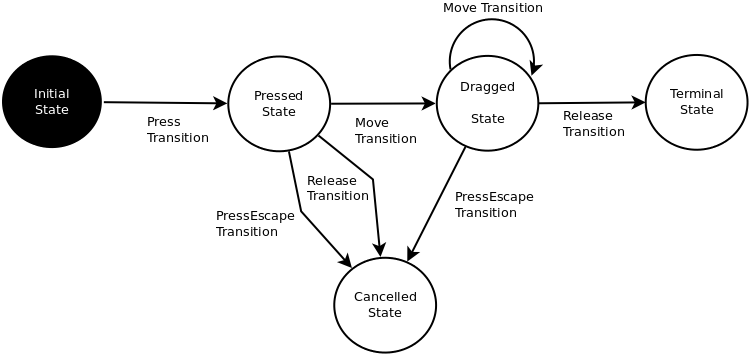
\includegraphics[height=6.0cm]{../assets/DnD.png}
                        \captionof{figure}{FSM du Drag and Drop}
                    \end{minipage}
                \vspace{0.5cm}
                \item Commande : Les commandes sont des actions qui seront appelée quand l'interaction utilisateur qui leur sont liée sera effectuée.
                MalaiTS possède les commandes de base courantes, mais permet de très facilement implémenter des commandes personnalisées.
                \vspace{0.2cm}
                \item Binder : Ce système est l'intérêt principal de Malai, il permet de lier une commande avec une interaction, tous en pouvant paramétrer le binder.
                Comme par exemple en donnant une condition pour que la commande soit effectuée, ou bien en effectuant une commande à chaque fois que l'interaction utilisateur est mise à jour.
            \end{itemize}

    \end{appendices}

\end{document}
